\chapter{Геометрия однородного пространства}

\lectureoverview{Плоскостность — превосходное приближение к наблюдаемой Вселенной, но не принцип. Если, допуская кривизну, сохранить однородность и изотропию, возникают три односвязные пространственные геометрии: евклидова, сферическая и гиперболическая. Их метрики можно построить, исходя из того, как концентрические оболочки растут с расстоянием, а их кривизну можно проверять по угловым размерам и подсчётам объектов. Плоское пространство также может быть конечным, если его топология тороидальна. Наконец, если приписать любому из этих однородных пространств зависящий от времени масштабный множитель, получаются космологические метрики пространства-времени и закон Хаббла; динамика этого масштабного множителя должна следовать из общей теории относительности.}

\section{Плоскостность — наблюдение, а не принцип}

До сих пор мы считали пространство плоским и почти ничего не говорили о геометрии пространства-времени. Наблюдения оправдывают использование плоского пространства как очень хорошего приближения, но не возводят плоскостность в ранг закона. Измерения в действительности говорят нам лишь о том, что любой радиус кривизны должен быть велик по сравнению с исследованной нами областью. Пространство может быть в точности плоским, положительно искривлённым или отрицательно искривлённым. На масштабах, значительно превосходящих наблюдаемую область, мы пока не знаем, какое из этих описаний верно.

Поэтому мы ослабим одно предположение, сохранив другое. Мы не будем предполагать плоскостность, но по-прежнему будем предполагать, что пространство однородно и изотропно. Это рабочая гипотеза, а не предмет веры. Чтобы выяснить её следствия, мы примем её и выполним вычисления; затем сможем от неё отказаться и спросить, как вела бы себя иначе неоднородная Вселенная.

Однородность означает, что каждая точка имеет один и тот же геометрический характер. Наблюдатель, который перемещается в другое место и повторяет локальные геометрические эксперименты, получает те же результаты. Изотропия означает, что ни одно направление не является предпочтительным. Эти условия исключают почти любую искривлённую поверхность, которую обычно рисуют первой. Параболоид искривлён сильнее вблизи своей вершины, чем вдали от неё. У вытянутого эллипсоида геометрия на полюсах и в экваториальной области различна. Сфера с буграми, или поверхность Земли, если различать на ней горы и долины, искривлена, но не однородна. Космологический вопрос уже:
\begin{quote}
Какие пространства могут быть искривлёнными и при этом выглядеть геометрически одинаково из каждой точки и во всех направлениях?
\end{quote}

Если пока не учитывать глобальные отождествления, то существуют три ответа с постоянной кривизной: плоское пространство, сферическое пространство положительной кривизны и гиперболическое пространство отрицательной кривизны. Эта оговорка о глобальных отождествлениях существенна; позже мы построим плоский конечный тор и исправим чрезмерно упрощённое утверждение, будто эти три случая исчерпывают все возможности.

\section{Метрика и координаты наблюдателя}

Сначала мы обсудим только пространство, а не пространство-время. Его геометрия закодирована в метрике: правиле для квадрата расстояния \(ds^2\) между соседними точками. Как только это локальное правило известно всюду, из него можно восстановить длины, углы, площади, объёмы, геодезические линии и кривизну.

Для евклидовой плоскости и трёхмерного евклидова пространства декартовы координаты дают
\begin{equation}
ds_2^2=dx^2+dy^2,
\qquad
ds_3^2=dx^2+dy^2+dz^2.
\label{eq:c03-cartesian-flat}
\end{equation}
Добавление третьего измерения просто добавляет ортогональный член \(dz^2\), но важна не простота этой формулы. Важно то, что уравнение~\eqref{eq:c03-cartesian-flat} полностью задаёт локальную геометрию.

\begin{figure}[htbp]
\centering
\includegraphics[width=0.74\textwidth]{lecture_03_figure_02.png}
\caption{Декартова метрика плоского трёхмерного пространства в том виде, как она записана на доске.}
\label{fig:c03-cartesian-board}
\lectureframe{00:05:13.138}
\end{figure}

Декартовы координаты скрывают то, как астроном воспринимает Вселенную. Мы находимся в одной точке, смотрим вовне в разных направлениях и упорядочиваем всё, что видим, по углу и расстоянию. В двумерной Вселенной поле зрения буквально было бы кругом направлений вокруг нас. Поэтому полярные координаты не просто изящны; они выявляют угловую геометрию, которой пользуется космология.

Пусть \(r\) — радиальное расстояние, а \(\theta\) — направление. Тогда та же самая евклидова плоскость имеет метрику
\begin{equation}
ds^2 = dr^2 + r^2 d\theta^2.
\label{eq:c03-polar-flat}
\end{equation}
При фиксированном малом угле \(d\theta\) поперечное расстояние равно \(r\,d\theta\). Оно растёт линейно по мере того, как мы удаляемся наружу, и потому его вклад в метрику в квадрате равен \(r^2d\theta^2\).

Угловой член сам по себе является метрикой одномерного пространства. Окружность — это одномерная сфера, обозначаемая \(S^1\), и метрику единичной окружности принято записывать как
\begin{equation}
d\Omega_1^2 = d\theta^2,
\qquad\text{so that}\qquad
ds^2 = dr^2 + r^2 d\Omega_1^2.
\label{eq:c03-omega-one}
\end{equation}
На доске используется \(d\Omega^2\) без различимого нижнего индекса; словесное определение однозначно показывает, что имеется в виду \(d\Omega_1^2\).

\begin{figure}[htbp]
\centering
\includegraphics[width=0.74\textwidth]{lecture_03_figure_03.png}
\caption{Схема полярных координат и метрика плоского пространства. На доске написано \(d\Omega^2\); из объяснения ясно, что это метрика единичной окружности \(d\Omega_1^2=d\theta^2\).}
\label{fig:c03-polar-board}
\lectureframe{00:08:37.254}
\end{figure}

\begin{figure}[htbp]
\centering
\begin{tikzpicture}[scale=1.2]
\draw[->] (-1.2,0)--(1.8,0);
\draw[->] (0,-1.2)--(0,1.8);
\draw[thick] (0,0)--(1.3,1.1);
\draw (0.7,0.7) node[above] {$r$};
\draw (0.58,0) arc (0:40:0.58);
\draw (0.8,0.22) node {$\theta$};
\end{tikzpicture}
\caption{Аккуратная реконструкция полярных координат, центрированных на наблюдателе, используемых в уравнении~\eqref{eq:c03-omega-one}.}
\label{fig:c03-polar-redraw}
\end{figure}

\begin{classroomqa}
\audiencequestion{Действительно ли \(d\theta^2\) задаёт меру расстояния вдоль окружности?}
\lecturerresponse{Да. На единичной окружности длина дуги равна углу в радианах, так что соседние точки, разделённые на \(d\theta\), имеют квадрат внутреннего расстояния \(d\theta^2\). Длина окружности равна \(2\pi\), и интегрирование \(ds=d\theta\) по одному полному обходу даёт в точности \(2\pi\). Умножение на \(r^2\) увеличивает единичную окружность до оболочки радиуса \(r\) на плоскости. \lecturetimestamp{00:09:11--00:09:26}}
\end{classroomqa}

Слово \emph{внутренний} здесь существенно. Если вложить единичную окружность в евклидову плоскость, её можно описать уравнением
\begin{equation}
x^2 + y^2 = 1.
\end{equation}
Это уравнение описывает, как окружность расположена в большем пространстве. Оно не нужно обитателю, который может измерять только расстояния вдоль окружности. Мы могли бы изогнуть гибкое оптическое волокно в перекошенную замкнутую петлю, не растягивая его. Его вид на плоскости изменился бы, но его внутренняя длина и его метрика — нет. Равные приращения \(\theta\) по-прежнему соответствовали бы равным расстояниям вдоль волокна. Следовательно, геометрию нужно отделять от случайной формы, задаваемой вложением.

\begin{figure}[htbp]
\centering
\includegraphics[width=0.64\textwidth]{lecture_03_figure_04.png}
\caption{На доске сравниваются круглая единичная окружность и деформированная замкнутая петля. Если петлю изгибать без растяжения, обе имеют одну и ту же внутреннюю одномерную метрику.}
\label{fig:c03-intrinsic-board}
\lectureframe{00:10:34.205}
\end{figure}

\begin{figure}[htbp]
\centering
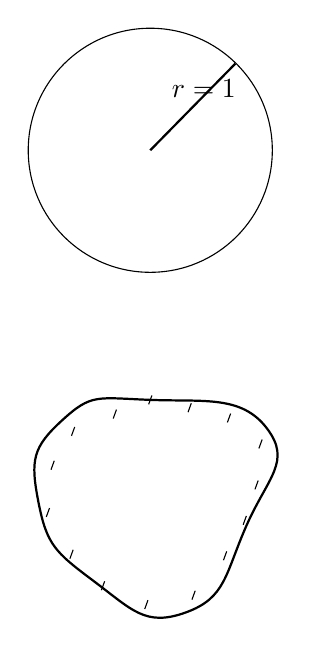
\begin{tikzpicture}[scale=1.0]
\draw (0,0) circle (1.55);
\draw[thick] (0,0)--(1.08,1.1);
\draw (0.68,0.78) node {$r=1$};

\begin{scope}[yshift=-4.35cm]
\draw[thick]
plot[smooth cycle, tension=0.95] coordinates
{(0,1.18) (1.48,0.82) (1.22,-0.42) (0.45,-1.52) (-0.72,-1.12) (-1.42,-0.12) (-1.12,0.92)};
\foreach \p in {(0,1.18),(0.5,1.08),(1.0,0.95),(1.4,0.62),(1.35,0.1),(1.2,-0.35),(0.95,-0.8),(0.55,-1.3),(-0.05,-1.42),(-0.6,-1.18),(-1.0,-0.78),(-1.3,-0.25),(-1.24,0.35),(-0.98,0.78),(-0.45,1.0)}{
\draw[rotate around={70:\p}] \p ++(-0.06,0) -- ++(0.12,0);
}
\end{scope}
\end{tikzpicture}
\caption{Внутреннее расстояние сохраняется при внешней деформации: одномерный обитатель измеряет одну и ту же длину замкнутой кривой при любом из двух вложений.}
\label{fig:c03-intrinsic-redraw}
\end{figure}

Теперь плоское пространство можно рассматривать как семейство вложенных окружностей вокруг наблюдателя. Оболочка на расстоянии \(r\) есть копия единичной окружности, увеличенная в \(r\) раз, и именно это фиксирует множитель \(r^2d\Omega_1^2\).

\section{Положительная кривизна: замыкающиеся оболочки}

Сфера искривлена, но однородна: ни одна точка на идеально круглой сфере геометрически не выделена по сравнению с другой. Мы можем построить её метрику, не обращаясь к внешней трёхмерной картине. Представьте двумерных астрономов, которые живут на единичной \(2\)-сфере и помещают начало координат в точку, где находятся сами.

Окружность, находящаяся на малом геодезическом расстоянии \(r\) от них, мала. По мере увеличения \(r\) эти окружности растут, достигают наибольшей длины на полпути вокруг сферы, а затем уменьшаются, пока не стягиваются в антиподальной точке. Этот рост и это сжатие происходят по мере изменения \emph{расстояния}, а не во времени. На всём протяжении этого построения сфера статична.

Здесь \(r\) — угловое расстояние вдоль единичной сферы, а не евклидово расстояние от центра:
\[
0 \le r \le \pi.
\]
При \(r=0\) находится выбранное начало, при \(r=\pi/2\) — большая окружность на полпути вокруг сферы, а при \(r=\pi\) — антипод. Радиус оболочки теперь равен \(\sin r\), поэтому плоский множитель \(r^2\) заменяется на \(\sin^2r\):
\begin{equation}
d\Omega_2^2 = dr^2 + \sin^2 r\, d\Omega_1^2
            = dr^2 + \sin^2 r\, d\theta^2.
\label{eq:c03-two-sphere}
\end{equation}
Концы интервала и середина ведут себя в точности так, как требуется:
\begin{equation}
\sin 0=0,
\qquad
\sin\frac{\pi}{2}=1,
\qquad
\sin\pi=0.
\end{equation}
Следовательно, оболочки начинаются с нулевого размера, достигают максимального размера и вновь замыкаются.

\begin{figure}[htbp]
\centering
\includegraphics[width=0.82\textwidth]{lecture_03_figure_05.png}
\caption{Переход от вложенных окружностей в плоском пространстве к оболочкам на сфере. Нижняя формула в кадре частично закрыта; её словесный вывод даёт замену \(r^2\mapsto\sin^2r\) в уравнении~\eqref{eq:c03-two-sphere}.}
\label{fig:c03-spherical-board}
\lectureframe{00:16:11.701}
\end{figure}

\begin{figure}[htbp]
\centering
\resizebox{\linewidth}{!}{%
\begin{tikzpicture}[scale=0.92]
\begin{scope}[xshift=-4.15cm]
\draw[->] (-1.7,0)--(1.9,0);
\draw[->] (0,-1.7)--(0,1.9);
\draw (0,0) circle (0.45);
\draw (0,0) circle (0.9);
\draw (0,0) circle (1.35);
\draw[thick] (0,0)--(1.45,1.2);
\draw (0.56,0.18) arc (18:40:0.63);
\draw (0.94,0.44) node {$\theta$};
\end{scope}

\begin{scope}[xshift=4.15cm]
\draw (0,0) circle (2.0);
\fill (0,-2.0) circle (1.5pt);
\fill (2.0,0) circle (1.5pt);
\fill (0,2.0) circle (1.5pt);
\draw[thick] (0,-2.0) arc (-90:90:2.0);
\draw (0,-2.35) node {$r=0$};
\draw (2.75,0) node {$r=\pi/2$};
\draw (0,2.35) node {$r=\pi$};
\end{scope}
\end{tikzpicture}
}%
\caption{Плоские оболочки растут неограниченно, тогда как сферические оболочки возрастают до максимума при \(r=\pi/2\) и замыкаются при \(r=\pi\).}
\label{fig:c03-shells-flat-sphere}
\end{figure}

Обозначение \(d\Omega_2^2\) означает метрику единичной \(2\)-сферы, так же как \(d\Omega_1^2\) означает метрику её круговых оболочек. Та же рекурсивная конструкция работает и на одну размерность выше. При фиксированном радиусе в плоском трёхмерном пространстве окружающая нас оболочка — это \(2\)-сфера:
\begin{equation}
ds_{\text{flat},3}^2 = dr^2 + r^2 d\Omega_2^2.
\label{eq:c03-flat-three-polar}
\end{equation}
Если эти оболочки, то есть \(2\)-сферы, растут, а затем замыкаются с множителем \(\sin r\), получающееся пространство есть единичная \(3\)-сфера:
\begin{equation}
d\Omega_3^2 = dr^2 + \sin^2 r\, d\Omega_2^2.
\label{eq:c03-three-sphere}
\end{equation}
\(3\)-сферу трудно наглядно представить, потому что для её привычного вложения потребовалось бы четырёхмерное евклидово пространство. Однако метрика полна и не нуждается ни в какой картинке. Вокруг любого выбранного наблюдателя расположены вложенные друг в друга \(2\)-сферы; они растут до максимального размера, а затем сжимаются к антиподальной точке.

\begin{classroomqa}
\audiencequestion{Наблюдатель находится в центре сферы?}
\lecturerresponse{Наблюдатель находится в центре \emph{координатных оболочек}, а не в каком-то привилегированном геометрическом центре. Начало координат — это точка пространства, и любой другой наблюдатель может выбрать свою собственную точку в качестве \(r=0\) и получить ту же метрику. Однородность как раз и означает, что никакой такой выбор не является предпочтительным. \lecturetimestamp{00:19:21--00:20:27}}
\end{classroomqa}

Исключительно для наглядности единичную окружность и единичную \(2\)-сферу можно вложить в евклидовы пространства:
\begin{equation}
x^2+y^2=1,
\qquad
x^2+y^2+z^2=1.
\end{equation}
Эти уравнения описывают вложения, а не дополнительную физику. Муравей, ограниченный окружностью или сферой, может определить внутреннюю метрику, не обнаруживая окружающего евклидова пространства. Аналогично, \(S^3\) — это не обычный шар с загадочной границей. Это полное трёхмерное пространство, описываемое уравнением~\eqref{eq:c03-three-sphere}.

\section{Как кривизна меняет то, что мы видим}

Геометрия становится физикой лишь тогда, когда она изменяет наблюдение. Предположим, что поперечный диаметр объекта \(d\) известен, его радиальное расстояние \(r\) было независимо определено, а на небе измерен его угловой диаметр \(d\theta\). Галактики дают лишь грубый интуитивный пример; в более точной космологии используют откалиброванные стандартные линейки и стандартные свечи. Информацию о расстоянии можно получить из спектрального красного смещения, соотношения Хаббла, светимости и взаимной калибровки различных классов объектов.

В плоском пространстве будем считать \(r\) постоянным по всему поперечному размеру объекта. Уравнение~\eqref{eq:c03-polar-flat} даёт
\begin{equation}
d^2 = r^2 d\theta^2.
\label{eq:c03-flat-angle-step}
\end{equation}
Следовательно,
\begin{equation}
d\theta = \frac{d}{r}.
\label{eq:c03-flat-angle}
\end{equation}
Угловой размер убывает обратно пропорционально расстоянию.

На единичной сфере поперечный размер оболочки равен \(\sin r\), а не \(r\):
\begin{equation}
d^2 = \sin^2 r\, d\theta^2,
\qquad\text{hence}\qquad
d\theta = \frac{d}{\sin r}.
\label{eq:c03-spherical-angle}
\end{equation}
При \(0<r<\pi\) имеем \(\sin r<r\), поэтому один и тот же объект на одном и том же радиальном расстоянии выглядит больше, чем в плоском пространстве. Его угловой размер сначала уменьшается, достигает минимума на экваторе, а затем увеличивается по мере того, как оболочка сжимается. В предельной идеализации в антиподальной точке все направления сходятся, и изображение растягивается по всему небу.

\begin{classroomqa}
\audiencequestion{Это та же идея, которую используют, чтобы определить кривизну по космическому микроволновому фону?}
\lecturerresponse{Да. Ранняя плазма задаёт характерный физический масштаб благодаря своим акустическим осцилляциям. Мы измеряем угол, под которым видна эта стандартная линейка, и сравниваем его с углом, предсказываемым каждой геометрией. Объекты не обязаны буквально быть галактиками; существенно именно сравнение известного поперечного масштаба с его наблюдаемым угловым размером. \lecturetimestamp{00:37:37--00:38:12}}
\end{classroomqa}

Объёмы оболочек дают второй тест. В трёхмерном плоском пространстве площадь оболочки пропорциональна \(r^2\); на единичной \(3\)-сфере — \(\sin^2r\). Поэтому в однородной совокупности число объектов на сферической оболочке сначала растёт с расстоянием, а после экватора уменьшается. Положительная кривизна предсказывает по сравнению с плоским пространством парную сигнатуру: достаточно далёкие стандартные линейки кажутся слишком большими, а в достаточно далёких оболочках объектов слишком мало.

\begin{figure}[htbp]
\centering
\resizebox{\linewidth}{!}{%
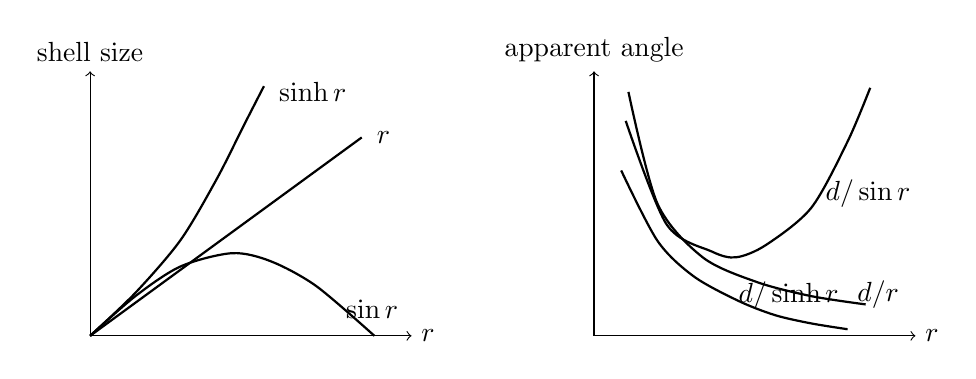
\begin{tikzpicture}[x=1.15cm,y=1.05cm]
\begin{scope}
\draw[->] (0,0)--(3.55,0) node[right] {$r$};
\draw[->] (0,0)--(0,3.2) node[above] {shell size};

\draw[thick] (0,0)--(3.0,2.4);
\draw (3.06,2.4) node[right] {$r$};

\draw[thick]
plot[smooth] coordinates {(0,0) (0.5,0.48) (1.0,0.84) (1.57,1.0) (2.0,0.9) (2.5,0.6) (3.14,0)};
\draw (2.72,0.55) node[below right] {$\sin r$};

\draw[thick]
plot[smooth] coordinates {(0,0) (0.5,0.52) (1.0,1.16) (1.4,1.9) (1.7,2.55) (1.92,3.02)};
\draw (1.98,2.95) node[right] {$\sinh r$};
\end{scope}

\begin{scope}[xshift=6.4cm]
\draw[->] (0,0)--(3.55,0) node[right] {$r$};
\draw[->] (0,0)--(0,3.2) node[above] {apparent angle};

\draw[thick]
plot[smooth] coordinates {(0.38,2.95) (0.7,1.6) (1.2,0.95) (1.8,0.65) (2.4,0.48) (3.0,0.38)};
\draw (2.8,0.5) node[right] {$d/r$};

\draw[thick]
plot[smooth] coordinates {(0.35,2.6) (0.8,1.35) (1.3,1.02) (1.57,0.95) (1.9,1.1) (2.4,1.55) (2.8,2.35) (3.05,3.0)};
\draw (2.45,1.72) node[right] {$d/\sin r$};

\draw[thick]
plot[smooth] coordinates {(0.3,2.0) (0.7,1.15) (1.1,0.72) (1.6,0.42) (2.0,0.25) (2.4,0.15) (2.8,0.08)};
\draw (2.15,0.2) node[above] {$d/\sinh r$};
\end{scope}
\end{tikzpicture}
}%
\caption{Радиальные множители для оболочек и соответствующие законы углового размера. Положительная кривизна заставляет оболочку замыкаться; отрицательная кривизна приводит к её экспоненциальному росту.}
\label{fig:c03-shell-angular-laws}
\end{figure}

\begin{classroomqa}
\audiencequestion{Становится ли радиальная координата бесконечной, если продолжать двигаться по сфере дальше?}
\lecturerresponse{Нет. На единичной сфере \(r\) — это геодезическое угловое расстояние, и оно принимает значения только от \(0\) до \(\pi\). При \(r=\pi\) оболочка схлопывается в антиподе. Здесь мы рассматриваем фиксированную пространственную геометрию, а не следим за объектом, который удаляется со временем. Позднее введение радиуса кривизны умножает все физические расстояния на этот радиус, но не изменяет этот безразмерный диапазон. \lecturetimestamp{00:39:30--00:40:35}}
\end{classroomqa}

\section{Проекция — не геометрия}

Прежде чем переходить к отрицательной кривизне, полезно увидеть, насколько сильно рисунок может исказить даже правильную геометрию. Поместим сферу на плоскость, касательную к ней в южном полюсе. Проведём прямую от северного полюса через каждую точку \(P\) на сфере и продолжим её до пересечения с плоскостью в \(P'\). Это стереографическая проекция. Сам северный полюс при этом отображается в бесконечность. Небольшая область вблизи южного полюса изображается с малым искажением, тогда как одинаковые по внутренней геометрии области вблизи северного полюса становятся на плоскости огромными.

Искажение относится к карте, а не к сфере. Исходная сфера остаётся однородной, хотя её плоское изображение приписывает эквивалентным областям крайне разные координатные размеры. Эта осторожность снова потребуется, когда бесконечное гиперболическое пространство будет сжато в конечный диск.

\begin{figure}[htbp]
\centering
\resizebox{\linewidth}{!}{%
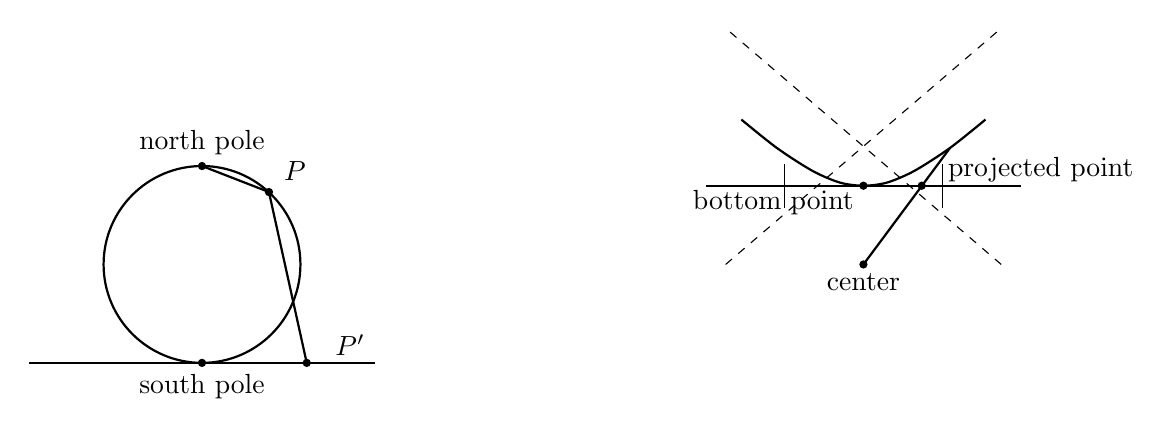
\begin{tikzpicture}[scale=1.0]
\begin{scope}[xshift=-4.2cm]
\draw[thick] (-2.2,-1.25)--(2.2,-1.25);
\draw[thick] (0,0) circle (1.25);
\fill (0,1.25) circle (1.5pt);
\fill (0,-1.25) circle (1.5pt);
\draw (0,1.55) node {north pole};
\draw (0,-1.55) node {south pole};

\fill (0.85,0.92) circle (1.5pt);
\draw (0.92,1.18) node[right] {$P$};
\draw[thick] (0,1.25)--(0.85,0.92)--(1.33,-1.25);
\fill (1.33,-1.25) circle (1.5pt);
\draw (1.57,-1.03) node[right] {$P'$};
\end{scope}

\begin{scope}[xshift=4.2cm]
\draw[thick] (-2.0,1)--(2.0,1);
\draw[dashed] (-1.75,0)--(1.75,3.0);
\draw[dashed] (1.75,0)--(-1.75,3.0);
\draw[thick]
plot[smooth] coordinates
{(-1.55,1.84) (-1.1,1.48) (-0.65,1.19) (-0.3,1.04) (0,1.0) (0.3,1.04) (0.65,1.19) (1.1,1.48) (1.55,1.84)};
\fill (0,0) circle (1.5pt);
\fill (0,1) circle (1.5pt);
\draw (0,-0.22) node {center};
\draw (0,0.78) node[left] {bottom point};
\draw[thick] (0,0)--(1.1,1.48);
\fill (0.74,1.0) circle (1.5pt);
\draw (0.95,1.2) node[right] {projected point};
\draw (-1,0.72) -- (-1,1.28);
\draw (1,0.72) -- (1,1.28);
\end{scope}
\end{tikzpicture}
}%
\caption{Слева: стереографическая проекция переводит северный полюс сферы в бесконечность. Справа: гиперболоид можно спроецировать на конечный диск, представленный здесь отрезком поперечного сечения. Координатное искажение не разрушает внутреннюю однородность.}
\label{fig:c03-projections}
\end{figure}

\section{Отрицательная кривизна: оболочки, растущие быстрее, чем в плоском пространстве}

Третья односвязная однородная геометрия заменяет \(\sin r\) на гиперболический синус. Её метрики в двух и трёх измерениях при единичном радиусе кривизны имеют вид
\begin{equation}
dh_2^2 = dr^2 + \sinh^2 r\, d\Omega_1^2,
\label{eq:c03-hyperbolic-two}
\end{equation}
\begin{equation}
dh_3^2 = dr^2 + \sinh^2 r\, d\Omega_2^2.
\label{eq:c03-hyperbolic-three}
\end{equation}
Координата \(r\) теперь принимает значения
\begin{equation}
0\le r<\infty.
\end{equation}
Вблизи начала координат \(\sinh r\approx r\), так что геометрия локально евклидова. Вдали её оболочки растут гораздо быстрее евклидовых и никогда не начинают уменьшаться.

Закон роста следует из
\begin{equation}
\sin r = \frac{e^{ir}-e^{-ir}}{2i},
\qquad
\sinh r = \frac{e^r-e^{-r}}{2}.
\label{eq:c03-sin-sinh}
\end{equation}
При больших \(r\) \(\sinh r\sim e^r/2\). Поэтому в двух измерениях длина окружности растёт с радиусом экспоненциально; в трёх измерениях площадь оболочки растёт как \(\sinh^2r\sim e^{2r}/4\). В однородном распределении на далёкой оболочке поэтому находится соответственно больше объектов.

Для поперечного объекта размера \(d\),
\begin{equation}
d^2 = \sinh^2 r\, d\theta^2,
\qquad\text{so}\qquad
d\theta = \frac{d}{\sinh r}.
\label{eq:c03-hyperbolic-angle}
\end{equation}
При больших значениях \(r\),
\begin{equation}
d\theta \sim 2d\,e^{-r}.
\end{equation}
Следовательно, отрицательная кривизна даёт признак, противоположный положительной кривизне: далёкие стандартные линейки кажутся слишком маленькими, а далёкие оболочки содержат слишком много объектов по сравнению с плоским пространством.

\begin{classroomqa}
\audiencequestion{Как по диапазонам радиальной координаты различить сферическое и гиперболическое пространство?}
\lecturerresponse{На единичной сфере \(r\) доходит до антипода, \(r=\pi\). В гиперболическом пространстве она продолжается без границ, \(0\le r<\infty\). Множитель оболочки выявляет тот же контраст: \(\sin r\) снова обращается в нуль, тогда как \(\sinh r\) растёт неограниченно. \lecturetimestamp{00:52:46--00:53:25}}
\end{classroomqa}

Существует вложение, которое делает однородность менее загадочной. Введём координаты окружающего пространства \(T,x,y\), где \(T\) — лишь координата вложения и \emph{не} космологическое время, и выберем верхний лист
\begin{equation}
T^2 - x^2 - y^2 = 1.
\label{eq:c03-hyperboloid}
\end{equation}
Наделим окружающее пространство метрикой лоренцевой сигнатуры
\begin{equation}
d\ell_{\mathrm{emb}}^2=-dT^2+dx^2+dy^2.
\label{eq:c03-ambient-minkowski}
\end{equation}
Метрика, индуцированная на гиперболоиде, положительно определена. Преобразования Лоренца сохраняют оба уравнения~\eqref{eq:c03-hyperboloid} и~\eqref{eq:c03-ambient-minkowski} и могут переводить любую точку верхнего листа в любую другую. В этом смысле смена начала координат в гиперболическом пространстве подобна наклону временной оси во вспомогательном окружающем пространстве. Все точки геометрически эквивалентны.

Спроецируем гиперболоид на диск, и бесконечно удалённые точки будут сгущаться у граничной окружности. Близкие области изображаются почти без искажений; более далёкие области сжимаются всё сильнее. Это дисковое представление Poincar\'e, знакомое по повторяющимся рисункам ангелов и чертей. Преобразование координат может перенести кажущуюся крошечной фигуру у края в центр, где она станет большой, сохраняя при этом все собственные длины и углы. В трёх измерениях соответствующая модель представляет собой шар, а не диск. Названия \emph{Poincar\'eпространство}, \emph{пространство Лобачевского} и \emph{пространство постоянной отрицательной кривизны} относятся к одной и той же локальной геометрии.

\begin{classroomqa}
\audiencequestion{Похож ли конечный диск на диаграмму Пенроуза?}
\lecturerresponse{Он похож лишь в том ограниченном смысле, что бесконечная область представлена внутри конечного рисунка. Однако здесь диск представляет только пространство, а не пространство-время и не причинную бесконечность. Его граница находится бесконечно далеко во внутренней гиперболической метрике, хотя на рисунке она помещена при конечном координатном радиусе. \lecturetimestamp{01:02:55--01:03:05}}
\end{classroomqa}

\section{Радиус кривизны}

Метрики, записанные до сих пор, описывают геометрии единичного радиуса кривизны. Чтобы придать сфере или гиперболическому пространству произвольный радиус кривизны, нужно умножить каждую длину на постоянную. На доске эта постоянная обозначена как \(a\); чтобы не путать её с зависящим от времени космологическим масштабным фактором, который будет использоваться позже, будем обозначать статический радиус кривизны через \(R_c\). Поскольку метрика измеряет квадрат длины,
\begin{align}
ds_{\mathrm{sph}}^2
  &=R_c^2d\Omega_n^2
   =R_c^2\left(dr^2+\sin^2r\,d\Omega_{n-1}^2\right),\\
ds_{\mathrm{hyp}}^2
  &=R_c^2dh_n^2
   =R_c^2\left(dr^2+\sinh^2r\,d\Omega_{n-1}^2\right).
\label{eq:c03-scaled-curvature}
\end{align}
Физическое радиальное расстояние равно \(R_cr\). Увеличение \(R_c\) делает пространство менее искривлённым; модуль постоянной секционной кривизны масштабируется как \(1/R_c^2\). В пределе \(R_c\to\infty\) обе искривлённые метрики на любой фиксированной конечной области переходят в евклидову геометрию.

\begin{classroomqa}
\audiencequestion{Если сделать сферу вдвое больше, станет ли она более искривлённой или менее искривлённой?}
\lecturerresponse{Менее искривлённой. Первый ответ, прозвучавший в аудитории, исправили, сравнив баскетбольный мяч с Землёй: меньшая поверхность изгибается быстрее на данном расстоянии. Удвоение \(R_c\) вдвое уменьшает масштаб кривизны, задаваемый обратным радиусом, и делит секционную кривизну \(1/R_c^2\) на четыре. \lecturetimestamp{01:10:14--01:10:56}}
\end{classroomqa}

Это объясняет, почему вблизи все три геометрии выглядят одинаково. При \(r\ll1\),
\begin{equation}
\sin r=r-\frac{r^3}{6}+\cdots,
\qquad
\sinh r=r+\frac{r^3}{6}+\cdots.
\end{equation}
В обеих искривлённых метриках ведущим членом является плоская полярная метрика; кривизна впервые проявляется через поправки относительного порядка \((L/R_c)^2\) на физическом масштабе \(L\).

\begin{classroomqa}
\audiencequestion{Говорят ли наблюдения, является ли пространство плоским, сферическим или гиперболическим?}
\lecturerresponse{Они показывают, что наблюдаемая область очень близка к плоской. Грубая оценка, сделанная на лекции, состояла в том, что ограничение на эффекты кривизны на уровне одного процента означает, что \(R_c\) как минимум примерно в десять раз больше размера видимой области, поскольку \((L/R_c)^2\lesssim10^{-2}\). Тогда соответствующий объём кривизны был бы как минимум порядка \(10^3\) видимых объёмов. Это оценка по порядку величины, сделанная на лекции, а не цитата из современных точных данных, и случай точной плоскостности \(R_c=\infty\) остаётся возможным. \lecturetimestamp{01:11:00--01:13:37}}
\end{classroomqa}

\section{Плоское, но конечное: тор}

Теперь мы должны исправить утверждение о том, что плоское, сферическое и гиперболическое пространства — единственные однородные варианты. Это три односвязные геометрии постоянной кривизны. Плоское пространство также может иметь нетривиальную глобальную топологию.

Начнём с евклидова прямоугольника. Отождествим его левый край поточечно с правым, а нижний край — с верхним. Пересекая любой край, вы возвращаетесь через противоположный. Локальная метрика остаётся \(dx^2+dy^2\), но глобально пространство периодично и конечно. Это факторпространство есть плоский двумерный тор \(T^2\). Одна периодическая размерность даёт окружность \(T^1\), отождествление противоположных граней прямоугольного параллелепипеда даёт плоский трёхмерный тор \(T^3\), и эта конструкция распространяется на любое число измерений.

\begin{figure}[htbp]
\centering
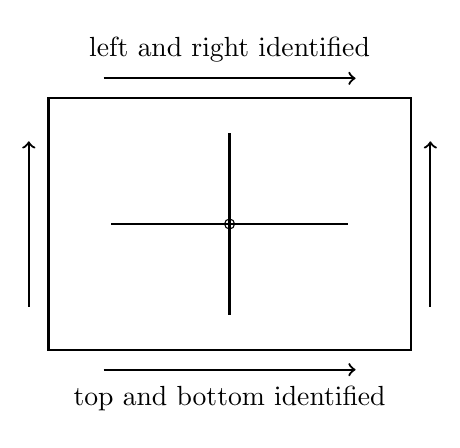
\begin{tikzpicture}[scale=1.0]
\draw[thick] (0,0) rectangle (4.6,3.2);

\draw[->,thick] (0.7,3.45)--(3.9,3.45);
\draw[->,thick] (0.7,-0.25)--(3.9,-0.25);

\draw[->,thick] (-0.25,0.55)--(-0.25,2.65);
\draw[->,thick] (4.85,0.55)--(4.85,2.65);

\draw[thick] (0.8,1.6)--(3.8,1.6);
\draw[thick] (2.3,0.45)--(2.3,2.75);

\draw (2.3,1.6) circle (1.8pt);

\draw (2.3,-0.62) node {top and bottom identified};
\draw (2.3,3.82) node {left and right identified};
\end{tikzpicture}
\caption{Плоский тор, построенный отождествлением противоположных сторон прямоугольника. Края не являются границами; попарно отождествлённые точки — это одни и те же точки факторпространства.}
\label{fig:c03-flat-torus}
\end{figure}

\begin{classroomqa}
\audiencequestion{Может ли Вселенная, следовательно, быть одновременно плоской и конечной?}
\lecturerresponse{Да. Плоскостность — это локальное утверждение о метрике; конечность может быть глобальным утверждением о топологии. Достаточно большой трёхмерный тор выглядел бы евклидовым во всей области, которую мы можем наблюдать, хотя его полный объём конечен. \lecturetimestamp{01:13:37--01:17:59}}
\end{classroomqa}

Картина универсального накрытия делает наблюдаемое следствие наглядным. Вместо отождествления краёв замостите бесконечную евклидову плоскость копиями фундаментального прямоугольника. Один и тот же объект в торе появляется по одному разу в каждой копии. В трёх измерениях эти копии образуют периодический кристаллоподобный массив.

\begin{classroomqa}
\audiencequestion{Могли бы мы жить в тороидальной Вселенной и не замечать этого?}
\lecturerresponse{Да, если фундаментальная ячейка больше области, из которой свет достиг нас. Если бы она была достаточно мала, свет мог бы пройти через эти отождествления, и мы увидели бы повторяющиеся изображения одних и тех же галактик, возможно даже повторяющиеся виды нашей собственной окрестности, в разных направлениях. Локальная геометрия в обоих случаях оставалась бы плоской. \lecturetimestamp{01:18:16--01:22:04}}
\end{classroomqa}

\begin{classroomqa}
\audiencequestion{Почему сфера заканчивается на антиподе, тогда как тор повторяется?}
\lecturerresponse{На сфере окружающая оболочка действительно сжимается до нуля при \(r=\pi\); все радиальные направления сходятся в антиподе. На торе край выбранной прямоугольной ячейки никогда не сжимается. Он отождествлён с противоположным краем того же размера, так что его пересечение продолжает то же пространство в периодическом координатном описании. \lecturetimestamp{01:22:06--01:23:02}}
\end{classroomqa}

\section{От пространства к пространству-времени}

Теперь мы можем вернуть время. В единицах, где скорость света \(c=1\), метрика Минковского имеет вид
\begin{equation}
ds^2 = -dt^2 + dx^2 + dy^2 + dz^2.
\label{eq:c03-minkowski}
\end{equation}
Выбор знаков — вопрос соглашения; существенно лишь то, что временной член имеет знак, противоположный пространственным членам. Световой луч следует по нулевой траектории,
\begin{equation}
ds^2 = 0.
\end{equation}
Для движения только вдоль \(x\),
\begin{equation}
-dt^2 + dx^2 = 0
\qquad\Rightarrow\qquad
dx = \pm dt.
\label{eq:c03-null-flat}
\end{equation}
Два знака описывают свет, движущийся влево или вправо с единичной скоростью.

В космологии мы сохраняем член собственного времени \(-dt^2\), заменяем евклидову пространственную часть на однородную пространственную метрику и позволяем её общему масштабу меняться со временем. Этот масштабный фактор мы обозначаем как \(a(t)\). Теперь это динамическая функция, а не фиксированный радиус \(R_c\), использовавшийся в статическом сравнении.

В качестве наглядного \(2+1\)-мерного примера возьмём
\begin{equation}
ds^2 = -dt^2 + a(t)^2 d\Omega_2^2.
\label{eq:c03-two-plus-one}
\end{equation}
При каждом фиксированном \(t\) пространство представляет собой \(2\)-сферу радиуса \(a(t)\). Наслаивая эти сферы во времени, получаем пространство-время. Привычная \(3+1\)-мерная конструкция имеет вид
\begin{equation}
ds^2 = -dt^2 + a(t)^2 d\Sigma^2,
\label{eq:c03-frw-general}
\end{equation}
где \(d\Sigma^2\) — не зависящая от времени единичная пространственная метрика. Три односвязных случая таковы:
\begin{align}
\text{flat:}\quad
ds^2&=-dt^2+a(t)^2\left(dx^2+dy^2+dz^2\right),\label{eq:c03-frw-flat}\\
\text{spherical:}\quad
ds^2&=-dt^2+a(t)^2d\Omega_3^2,\label{eq:c03-frw-spherical}\\
\text{hyperbolic:}\quad
ds^2&=-dt^2+a(t)^2dh_3^2.\label{eq:c03-frw-hyperbolic}
\end{align}
Относительный масштаб сопутствующих координат фиксирован, тогда как \(a(t)\) меняется. В сферической и гиперболической нормировках \(a(t)\) также является мгновенным радиусом кривизны. В плоском случае его абсолютную нормировку можно поглотить в сопутствующие координаты.

Закон Хаббла получается ещё до введения какого-либо уравнения гравитационного поля. Рассмотрим две близкие сопутствующие точки с фиксированным координатным расстоянием \(\chi\). Их физическое расстояние равно
\begin{equation}
D(t)=a(t)\chi.
\label{eq:c03-comoving-distance}
\end{equation}
Дифференцируя при фиксированном \(\chi\), получаем
\begin{equation}
V=\dot D=\dot a(t)\chi.
\end{equation}
Исключая \(\chi\),
\begin{equation}
V = \frac{\dot a}{a} D.
\label{eq:c03-hubble-law}
\end{equation}
Следовательно,
\begin{equation}
H = \frac{\dot a}{a}.
\label{eq:c03-hubble-parameter}
\end{equation}
Это кинематическое тождество для однородного расширения или сжатия. Оно верно для всех трёх пространственных геометрий: \(\dot a>0\) означает удаление, а \(\dot a<0\) — сближение.

Одна лишь геометрия не определяет \(a(t)\). Функции вида
\begin{equation}
a(t)\propto t^{2/3},
\qquad
a(t)\propto t^{1/2},
\qquad
a(t)\propto e^{Ht}
\end{equation}
все согласуются с анзацем однородной метрики, но описывают различное космическое содержание материи и энергии. Общая теория относительности даёт динамическое уравнение, которое выбирает между ними. Получающееся уравнение Фридмана также свяжет плоский, сферический и гиперболический случаи с вариантами ньютоновской космологии, рассмотренной ранее, с нулевой, отрицательной и положительной энергией.

\begin{classroomqa}
\audiencequestion{Могут ли геометрия и космическая эволюция быть намного сложнее, чем в этих моделях?}
\lecturerresponse{Разумеется. Однородность и изотропия — ограничительные предположения, выбранные потому, что они естественны, хорошо согласуются с наблюдениями на больших масштабах и математически поддаются анализу. Существует множество более сложных геометрий и эволюций. Важный динамический вопрос состоит в том, эволюционируют ли широкие классы изначально нерегулярных моделей к одной из этих простых однородных форм. \lecturetimestamp{01:36:00--01:36:50}}
\end{classroomqa}

\begin{classroomqa}
\audiencequestion{Является ли \(3\)-сфера границей четырёхмерного объекта?}
\lecturerresponse{Так её можно представить как вложение, но космологическое пространство — это сама \(3\)-сфера. У неё три внутренних измерения и нет границы. Четырёхмерная евклидова картинка — лишь необязательная вспомогательная конструкция; уравнение~\eqref{eq:c03-three-sphere} уже полностью определяет геометрию. \lecturetimestamp{01:36:55--01:37:59}}
\end{classroomqa}

\begin{classroomqa}
\audiencequestion{Является ли светимость единственным способом получить расстояние, нужное для проверки кривизны?}
\lecturerresponse{Нет. Спектральные линии определяют красное смещение, близкие ступени лестницы расстояний калибруют соотношение Хаббла, а сверхновые дают приблизительно стандартные светимости. Эти методы взаимно проверяются, а не принимаются на веру по отдельности. Даже закон обратных квадратов для светимости зависит от геометрии, потому что площадь светового фронта задаётся \(r^2\), \(\sin^2r\) или \(\sinh^2r\). Именно согласие нескольких наблюдаемых величин поддерживает вывод о почти плоской геометрии. \lecturetimestamp{01:38:00--01:41:07}}
\end{classroomqa}

\section{Что следует запомнить}

Геометрию однородной Вселенной можно определить по тому, как растут оболочки вокруг любого наблюдателя:
\begin{equation}
f(r)=
\begin{cases}
r, & \text{flat space},\\
\sin r, & \text{positive curvature},\\
\sinh r, & \text{negative curvature}.
\end{cases}
\end{equation}
Пространственная метрика имеет вид \(dr^2+f(r)^2d\Omega_{n-1}^2\). Та же функция управляет угловыми размерами и числом объектов на оболочке, поэтому кривизна имеет прямой наблюдательный смысл. Большой радиус кривизны локально скрывает эти различия, а тороидальное отождествление показывает, что одна только локальная кривизна не определяет глобальный размер или топологию.

Добавление \(-dt^2\) и общего множителя \(a(t)^2\) превращает любую из трёх однородных пространственных метрик в космологическое пространство-время. Отсюда сразу следует \(V=HD\) при \(H=\dot a/a\), но \(a(t)\) при этом остаётся неопределённым. Поэтому следующий шаг — уже не очередное геометрическое упражнение. Это динамическая задача: использовать уравнения Эйнштейна, чтобы определить, как вещество, излучение, кривизна и другие формы энергии заставляют масштабный фактор эволюционировать.
